\chapter{Новые результаты}



Попробовал посчитать с перебором $M_{k1}$ и $M_{k2}$, так как для  всех 4 критериев кривые почти сливаются, как и в ваших расчетах, где отдельно отстоят кривая 3 (оптимумы по массе высокообогащенной фракции) и кривая 5: минимум концентрации $^{236}$U\dots




\begin{figure}
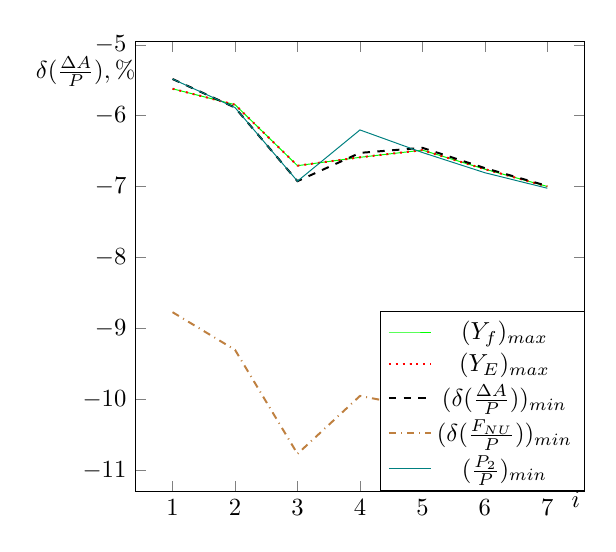
\begin{tikzpicture}[,
scale=0.89]
\begin{axis}[
  xlabel style = {{at={(axis description cs:.98,0.02)}}},
  ylabel = {$\delta(\frac{\Delta A}{P}), \%$},
  ylabel style = {{at={(axis description cs:-0.11,.88)},rotate=270,anchor=south}},
  xlabel = {$i$},
  width=8cm, height=8cm, xtick={1,2,3,4,5,6,7}, legend style={at={(1,0)},anchor=south east}
]

\addplot+[mark=none,
  solid, green, thin
] coordinates {
  (1.0, -5.619564224321039)
  (2.0, -5.84441657242741)
  (3.0, -6.704917867424845)
  (4.0, -6.586866390801599)
  (5.0, -6.485554729454776)
  (6.0, -6.754284481908828)
  (7.0, -6.998000929961407)
};
\addlegendentry{{}{$(Y_f)_\text{max}$}}

\addplot+[mark=none,
  dotted, red, thick
] coordinates {
  (1.0, -5.619564224321039)
  (2.0, -5.84441657242741)
  (3.0, -6.704917867424845)
  (4.0, -6.586866390801599)
  (5.0, -6.485554729454776)
  (6.0, -6.754284481908828)
  (7.0, -6.998000929961407)
};
\addlegendentry{{}{$(Y_{E})_\text{max}$}}

\addplot+[mark=none,
  dashed, black, thick
] coordinates {
  (1.0, -5.482150178426482)
  (2.0, -5.884813687357447)
  (3.0, -6.923308229121754)
  (4.0, -6.524186589001574)
  (5.0, -6.4527000666451135)
  (6.0, -6.739088245807983)
  (7.0, -6.991066392896656)
};
\addlegendentry{{}{$(\delta(\frac{\Delta A}{P}))_\text{min}$}}

\addplot+[mark=none,
  dashdotted, brown, thick
] coordinates {
  (1.0, -8.771994897379303)
  (2.0, -9.303209789751323)
  (3.0, -10.770438360555245)
  (4.0, -9.953392791027085)
  (5.0, -10.122163189828624)
  (6.0, -10.411774829351534)
  (7.0, -10.654096806225095)
};
\addlegendentry{{}{$(\delta(\frac{F_{NU}}{P}))_\text{min}$}}

\addplot+[mark=none,
  solid, teal, thin
] coordinates {
  (1.0, -5.482150178426482)
  (2.0, -5.884813687357447)
  (3.0, -6.923308229121754)
  (4.0, -6.2006153993959785)
  (5.0, -6.519171025702167)
  (6.0, -6.804418040883925)
  (7.0, -7.023084861927327)
};
\addlegendentry{{}{$(\frac{P_2}{P})_\text{min}$}}

\end{axis}
\end{tikzpicture}


\caption{{Зависимость экономии работы разделения от номера перегрузки с обогащением на уровне 4,95\% для разных критериев оптимальности.{\label{loop_sw}}}}
\end{figure}


\begin{figure}
    \begin{tikzpicture}[,
scale=0.95]
\begin{axis}[
  xlabel style = {{at={(axis description cs:.86,0)}}},
  ylabel = {$Y_{f}, \%$},
  ylabel style = {{at={(axis description cs:-0.04,.95)},rotate=270,anchor=south}},
  xlabel = {$i$},
  width=16cm, height=16cm, xtick={1,2,3,4,5,6,7}
]

\addplot+[
  solid, green, thin
] coordinates {
  (1.0, 85.21609032233688)
  (2.0, 83.6193404447232)
  (3.0, 81.61368966907641)
  (4.0, 80.57950552353023)
  (5.0, 80.0845336767702)
  (6.0, 79.41378113072125)
  (7.0, 78.79089548101278)
};
\addlegendentry{{}{$(Y_f)_\text{max}$}}

\addplot+[
  dotted, red, thick
] coordinates {
  (1.0, 85.21609032233688)
  (2.0, 83.6193404447232)
  (3.0, 81.61368966907641)
  (4.0, 80.57950552353023)
  (5.0, 80.0845336767702)
  (6.0, 79.41378113072125)
  (7.0, 78.79089548101278)
};
\addlegendentry{{}{$(Y_{E})_\text{max}$}}

\addplot+[
  dashed, black, thick
] coordinates {
  (1.0, 85.38309104640025)
  (2.0, 83.64433144872015)
  (3.0, 81.41196203685915)
  (4.0, 80.53196741269147)
  (5.0, 80.0643020580487)
  (6.0, 79.40461693851607)
  (7.0, 78.78661478328848)
};
\addlegendentry{{}{$(\delta(\frac{\Delta A}{P}))_\text{min}$}}

\addplot+[
  dashdotted, brown, thick
] coordinates {
  (1.0, 85.36543264305068)
  (2.0, 83.58970595888829)
  (3.0, 81.56984369727179)
  (4.0, 80.72191929789999)
  (5.0, 80.0372154110709)
  (6.0, 79.32064929118525)
  (7.0, 78.67373437848555)
};
\addlegendentry{{}{$(\delta(\frac{F_{NU}}{P}))_\text{min}$}}

\addplot+[
  solid, teal, thin
] coordinates {
  (1.0, 85.38309104640025)
  (2.0, 83.64433144872015)
  (3.0, 81.41196203685915)
  (4.0, 80.92068234992644)
  (5.0, 80.16628140368758)
  (6.0, 79.44943999636384)
  (7.0, 78.8076611327759)
};
\addlegendentry{{}{$(\frac{P_2}{P})_\text{min}$}}

\end{axis}
\end{tikzpicture}


    \caption{{Зависимость экономии работы разделения от номера перегрузки с обогащением на уровне 4,95\% для разных критериев оптимальности.{\label{loop_ex}}}}
    \end{figure}

\begin{figure}
    \begin{tikzpicture}[,
scale=0.95,
scale=0.95]
\begin{axis}[
  xlabel style = {{at={(axis description cs:.86,0)}}},
  ylabel = {$R_{RepU}, \%$},
  ylabel style = {{at={(axis description cs:-0.08,.925)},rotate=270,anchor=south}},
  xlabel = {$i$},
  width=16cm, height=16cm
]

\addplot+[
  solid, black, thick
] coordinates {
  (1.0, 72.8241808435042)
  (2.0, 66.68566594907492)
  (3.0, 58.35228156487533)
  (4.0, 56.643420943442365)
  (5.0, 56.21679099162951)
  (6.0, 54.184876916297)
  (7.0, 52.553320781875414)
};
\addlegendentry{{}{$(R_f)_\text{max}$}}

\addplot+[
  dotted, black, thick
] coordinates {
  (1.0, 72.8241808435042)
  (2.0, 66.68566594907492)
  (3.0, 58.35228156487533)
  (4.0, 56.643420943442365)
  (5.0, 56.21679099162951)
  (6.0, 54.184876916297)
  (7.0, 52.553320781875414)
};
\addlegendentry{{}{$(R_{RepU})_\text{max}$}}

\addplot+[
  dashed, black, thick
] coordinates {
  (1.0, 73.82998902426432)
  (2.0, 66.64446941870102)
  (3.0, 57.19448148394325)
  (4.0, 56.67546946948041)
  (5.0, 56.226760998555434)
  (6.0, 54.188337945615274)
  (7.0, 52.5546392882073)
};
\addlegendentry{{}{$(\delta(\frac{\Delta U}{P}))_\text{min}$}}

\addplot+[
  dashdotted, black, thick
] coordinates {
  (1.0, 73.75583473104476)
  (2.0, 66.44811675745768)
  (3.0, 58.2996545335423)
  (4.0, 57.50685876177931)
  (5.0, 55.96223087076096)
  (6.0, 53.951506368752476)
  (7.0, 52.3277838935582)
};
\addlegendentry{{}{$(\delta(\frac{F_{NU}}{P}))_\text{min}$}}

\addplot+[
  solid, red, thick
] coordinates {
};
\addlegendentry{{}{$(C_{232,P})_\text{min}$}}

\addplot+[
  solid, blue, thick
] coordinates {
};
\addlegendentry{{}{$(C_{236,P})_\text{min}$}}

\addplot+[
  solid, brown, thick
] coordinates {
  (1.0, 73.82998902426432)
  (2.0, 66.64446941870102)
  (3.0, 57.19448148394325)
  (4.0, 58.460758694419646)
  (5.0, 56.177556015313)
  (6.0, 54.169304400774244)
  (7.0, 52.547895768556174)
};
\addlegendentry{{}{$(\frac{P_2}{P})_\text{min}$}}

\end{axis}
\end{tikzpicture}


    \caption{{Зависимость экономии работы разделения от номера перегрузки с обогащением на уровне 4,95\% для разных критериев оптимальности.{\label{loop_exR}}}}
    \end{figure}
    
    
    \begin{figure}
        \begin{tikzpicture}[,
scale=0.95]
\begin{axis}[
  xlabel style = {{at={(axis description cs:.86,0)}}},
  ylabel = {$\delta(\frac{F_{NU}}{P}), \%$},
  ylabel style = {{at={(axis description cs:-0.08,.94)},rotate=270,anchor=south}},
  xlabel = {$i$},
  width=16cm, height=16cm, xtick={1,2,3,4,5,6,7}
]

\addplot+[
  solid, green, thin
] coordinates {
  (1.0, 9.60224940765123)
  (2.0, 10.471964607421514)
  (3.0, 10.328677265019726)
  (4.0, 10.937722799772365)
  (5.0, 11.551073258460454)
  (6.0, 11.482634526238378)
  (7.0, 11.495414262020132)
};
\addlegendentry{{}{$(Y_f)_\text{max}$}}

\addplot+[
  dotted, red, thick
] coordinates {
  (1.0, 9.60224940765123)
  (2.0, 10.471964607421514)
  (3.0, 10.328677265019726)
  (4.0, 10.937722799772365)
  (5.0, 11.551073258460454)
  (6.0, 11.482634526238378)
  (7.0, 11.495414262020132)
};
\addlegendentry{{}{$(Y_{E})_\text{max}$}}

\addplot+[
  dashed, black, thick
] coordinates {
  (1.0, 9.758344663807906)
  (2.0, 10.377586059230682)
  (3.0, 10.148945832377942)
  (4.0, 11.036603656094378)
  (5.0, 11.596700175896046)
  (6.0, 11.502422364899322)
  (7.0, 11.5042389394856)
};
\addlegendentry{{}{$(\delta(\frac{\Delta A}{P}))_\text{min}$}}

\addplot+[
  dashdotted, brown, thick
] coordinates {
  (1.0, 10.428757919569875)
  (2.0, 11.091940883100326)
  (3.0, 11.132231272182302)
  (4.0, 11.940825541138867)
  (5.0, 12.240045586112991)
  (6.0, 12.233596137265634)
  (7.0, 12.281186997924387)
};
\addlegendentry{{}{$(\delta(\frac{F_{NU}}{P}))_\text{min}$}}

\addplot+[
  solid, teal, thin
] coordinates {
  (1.0, 9.758344663807906)
  (2.0, 10.377586059230682)
  (3.0, 10.148945832377942)
  (4.0, 11.415331124937522)
  (5.0, 11.403205816515582)
  (6.0, 11.411528711119201)
  (7.0, 11.462271406331004)
};
\addlegendentry{{}{$(\frac{P_2}{P})_\text{min}$}}

\end{axis}
\end{tikzpicture}


        \caption{{Зависимость экономии работы разделения от номера перегрузки с обогащением на уровне 4,95\% для разных критериев оптимальности.{\label{loop_pFo}}}}
        \end{figure}

\clearpage